\chapter{Abcd Framework}
\label{chap:abcd_frame}
In order to improve the \cite{ametrano_ballabio_mazzocchi} framework it is essential to understand the previous implementation, which is written in C++ language and available in the QuantLib library \cite{quantlib_dev}, ``experimental" folder, tenorbasis branch.

\section{Tenor Basis}
\textit{TenorBasis} is the super class from which the abcd scheme derives. It is modelled as a \textit{CalibratedModel}:

\begin{lstlisting}
class TenorBasis : public CalibratedModel{
  public:
    TenorBasis(Size nArguments,
               boost::shared_ptr<IborIndex> iborIndex,
               boost::shared_ptr<IborIndex> baseIborIndex,
               Date referenceDate = Date());
}
\end{lstlisting} 

such that it inherits its structure and methods, it sets the number of arguments (i.e. parameters) \textit{nArguments}, that the model needs to fit. Moreover, it adds features like the storing of a \textit{baseIborIndex}, which is the base curve with respect to search the \textit{TenorBasis}.
The most important methods for the basis calibration are:

\begin{lstlisting}
Rate accrualFactor(Date d1,Date d2) const;
\end{lstlisting} 

and

\begin{lstlisting}
void calibrate(
    const std::vector<boost::shared_ptr<RateHelper> >&,
    OptimizationMethod& method,
    const EndCriteria& endCriteria,
    const std::vector<Real>& weights = std::vector<Real>(),
    const std::vector<bool>& fixParameters;)
\end{lstlisting} 

For better understanding these two functions, it needs to be shown the curve underlying the bootstrapping procedure:

\begin{lstlisting}
class TenorBasisYieldTermStructure : public YieldTermStructure {
  public:
    TenorBasisYieldTermStructure(const boost::shared_ptr<TenorBasis>& basis);
    const Date& referenceDate() const;
    Calendar calendar() const;
    Natural settlementDays() const;
    Date maxDate() const;
    
  private:
    DiscountFactor discountImpl(Time) const;
    boost::shared_ptr<TenorBasis> basis_;
}
\end{lstlisting} 

and  its constructor:

\begin{lstlisting}
TenorBasisYieldTermStructure (const boost::shared_ptr<TenorBasis>& basis) : YieldTermStructure(basis->dayCounter()), basis_(basis) {}
\end{lstlisting} 

that simply builds an \textit{YieldTermStructure} object and stores a \textit{TenorBasis} object called basis in $basis\_$ (and implicitly also the base curve stored in $basis\_$). Moreover, it designs a \textit{discountImpl} which will be fundamental and therefore later explained.


The core of \textit{TenorBasis} is the \textit{calibrate} method which follows:

\begin{lstlisting}
void TenorBasis::calibrate(
    const std::vector<boost::shared_ptr<RateHelper> >& helpers,
    OptimizationMethod& method,
    const EndCriteria& endCriteria,
    const std::vector<Real>& weights,
    const std::vector<bool>& fixParameters) 
{
    TenorBasisYieldTermStructure 
    yts(boost::shared_ptr<TenorBasis>(this, no_deletion));
    std::vector<boost::shared_ptr<CalibrationHelperBase> > 
                                  cHelpers(helpers.size());
    for (Size i = 0; i<helpers.size(); ++i) {
        helpers[i]->setTermStructure(&yts);
        cHelpers[i] = helpers[i];
    }
    CalibratedModel::calibrate(cHelpers, method, endCriteria,
                       constraint(), weights, fixParameters);
}
\end{lstlisting} 

A \textit{TenorBasisYieldTermStructure}, which stores the \textit{TenorBasis} object itself as $basis\_$, is built and called yts (here it is possible to appreciate the design of the \textit{TenorBasisYieldTermStructure} previously explained). 
Subsequently, a vector of \textit{CalibrationHelperBase} is instantiated. It is fundamental the chain which links \textit{CalibrationHelperBase} and \textit{RateHelper}: indeed the latter inherits from \textit{BootstrapHelper}, which is child of \textit{CalibrationHelperBase} too. Given these chains of properties it is possible to write :
\begin{lstlisting}
cHelpers[i] = helpers[i]
\end{lstlisting}

Therefore, it is the first link between the general model \textit{CalibratedModel} and the specific implementation of \textit{TenorBasis}.
Moreover, the helpers are given a pointer to the yts, such that if they need to provide their quotes they use the pointed and bootstrapped term structure.
In the end the method from the parent class \textit{CalibratedModel} is exploited (note: C++ is capable of understanding what method to call depending on the type of parameters, which is the reason why it is necessary to cast from \textit{RateHelper} to \textit{CalibrationHelperBase}):

\begin{lstlisting}
void CalibratedModel::calibrate(
        const vector<shared_ptr<CalibrationHelperBase> >& h,
        OptimizationMethod& method,
        const EndCriteria& endCriteria,
        const Constraint& additionalConstraint,
        const vector<Real>& w,
        const vector<bool>& fixParameters) 
{

    //checks and problem setting...
    
    Problem prob(f, pc, proj.project(prms));
    shortRateEndCriteria_ = method.minimize(prob, endCriteria);
    Array result(prob.currentValue());
    setParams(proj.include(result));
    problemValues_ = prob.values(result);

    notifyObservers();
}
\end{lstlisting}

After have checked different steps, it sets the problem and asks the specific method to minimize it. The chosen one is \textit{LevenbergMarquardt}:

\begin{lstlisting}
EndCriteria::Type LevenbergMarquardt::minimize(Problem& P,const EndCriteria& endCriteria) 
{
    EndCriteria::Type ecType = EndCriteria::None;
    P.reset();
    Array x_ = P.currentValue();
    currentProblem_ = &P;
    initCostValues_ = P.costFunction().values(x_);
    int m = initCostValues_.size();
    int n = x_.size();
        
    //variables instantiation
        
    //error messages

    //set cost function
        
    //minimize through lmdif 
        
    std::copy(xx.get(), xx.get()+n, x_.begin());
    P.setCurrentValue(x_);
    P.setFunctionValue(P.costFunction().value(x_));

    return ecType;
}
\end{lstlisting}

It resets the problem and sets the initial variables. It performs a series of checks, it sets a particular cost function \textit{LevenbergMarquardt::fcn} and then \textit{lmdif} performs the minimization. Subsequently, the current problem value and the cost function one are set. 
Without being too specific, in \textit{lmdif} the errors that should be minimized are retrieved through the \textit{values} function embedded in the Levenberg Marquardt cost function:

\begin{lstlisting}
 void LevenbergMarquardt::fcn(int, int n, Real* x,Real* fvec, int*) 
 {
    Array xt(n);
    std::copy(x, x+n, xt.begin());
    if (currentProblem_->constraint().test(xt)) {
        const Array& tmp = currentProblem_->values(xt);
        std::copy(tmp.begin(), tmp.end(), fvec);
    } 
    else
    {
        std::copy(initCostValues_.begin(),
        initCostValues_.end(), fvec);
    }
}
\end{lstlisting}

The implementation of \textit{values}, from the \textit{model} class, follows:

\begin{lstlisting}
virtual Disposable<Array>values(const Array& params)const
{
    model_->setParams(projection_.include(params));
    Array values(helpers_.size());
    for (Size i=0; i<helpers_.size(); ++i) {
        values[i] = helpers_[i]->calibrationError() *
        std::sqrt(weights_[i]);
    }
    return values;
}
\end{lstlisting}

Here a fundamental role is played by:

\begin{lstlisting}
void CalibratedModel::setParams(const Array& params) 
{
    Array::const_iterator p = params.begin();
    for (Size i=0; i<arguments_.size(); ++i) {
        for (Size j=0; j<arguments_[i].size(); ++j, ++p) {
        ...
            arguments_[i].setParam(j, *p);
        }
    }
    QL_REQUIRE(p==params.end(),"parameter array too big!");
    generateArguments();
    notifyObservers();
}
\end{lstlisting}

Before asking the calibration error, this function sets the \textit{params} chosen by the algorithm in the \textit{arguments\_} container, that caches the parameters and allows to use them in \textit{generateArguments} in order to set the parameter to the specific model.The method \textit{generateArguments} is fundamental because links the general \textit{CalibratedModel} with the specific implementation of, in this case, \textit{AbcdTenorBasis} model and it allows to add the specific elements of the worked model (better explaied in \textit{AbcdTenorBasis} description). For this reason the further modifications will be performed here. 

In \textit{values}, the overall error is retrieved asking the helpers to retrieve its \textit{calibrationError()}, acting out the bootstrapping \textit{``à la QuantLib"} which creates an error, exploiting the polymorphic feature of the particular instantiated rate helper:

\begin{lstlisting}
helpers_[i]->calibrationError() 
\end{lstlisting}

\begin{lstlisting}
Real calibrationError() const {return quote_->value() - impliedQuote(); }
\end{lstlisting}

asking its \textit{TenorBasisYieldTermStructure} about the implied quote, for instance for a futures:

\begin{lstlisting}
Real FuturesRateHelper::impliedQuote() const 
{
    QL_REQUIRE(termStructure_ != 0, "term structure not set");
    Rate forwardRate = (termStructure_->discount(earliestDate_)
    /termStructure_->discount(maturityDate_) - 1.0) 
    / yearFraction_;
    Rate convAdj = convAdj_.empty() ? 0.0 : convAdj_->value();
    Rate futureRate = forwardRate + convAdj;
    return 100.0 * (1.0 - futureRate);
}
\end{lstlisting}

It is worth to know that the \textit{zeroRate} and \textit{forwardRate} functions in QuantLib are all implemented as functions of \textit{discount}, that is a function of \textit{disocuntImpl}, therefore they are linked.\\
The specific\textit{TenorBasisYieldTermStructure::discountImpl} is:

\begin{lstlisting}
DiscountFactor TenorBasisYieldTermStructure::discountImpl(Time t) const
{
    Date ref = referenceDate();
    Date d = basis_->dateFromTime(t);
    Real accrFactor = basis_->accrualFactor(ref, d);
    return 1.0 / accrFactor;
}
\end{lstlisting}

that depends on \textit{accrualFactor}, which models the pseudo discount with the abcd framework according to \eqref{eq:forward_from_adj_disc}:

\begin{lstlisting}
Rate TenorBasis::accrualFactor(Date d1,
                           Date d2) const
{
    QL_REQUIRE(d1 <= d2,
               "d2 (" << d2 << ") cannot be
               before d1 (" << d1 << ")");
    // baseCurve must be a discounting curve...
    // otherwise it could not provide fwd(t1, t2) with t2-t1!=tau
    Handle<YieldTermStructure> baseCurve =
    baseIborIndex_->forwardingTermStructure();
    Real accrFactor =
    baseCurve->discount(d1) / baseCurve->discount(d2);
    Real instContBasisIntegral = sign_ * integrate_(d1, d2);
    accrFactor *= std::exp(instContBasisIntegral);
    return accrFactor;
}
\end{lstlisting}

Therefore, the \textit{accrFactor} is initially retrieved from the \textit{baseCurve} through the \textit{discount} method and then multiplied by the compounding factor, where the exponential factor is the integrated instantaneous basis. Therefore, the problem consists in starting from a base curve expressed as discount factor reshaping it with a basis whom parameters are changed in order to minimize the overall error. Note: the sign of the abcd factor depends on whether or not we are calibrating with respect to a \textit{baseCurve} with a greater \textit{tenor} with respect to the benchmark curve whom base is searched.

\section{Abcd Tenor Basis}

\textit{AbcdTenorBasis} is a child class of the above presented \textit{TenorBasis}. Its constructor is: 

\begin{lstlisting}
AbcdTenorBasis::AbcdTenorBasis(shared_ptr<IborIndex> iborIndex,
                   boost::shared_ptr<IborIndex> baseIborIndex,
                   Date referenceDate,
                   bool isSimple,
                   const std::vector<Real>& coeff)
    : TenorBasis(4, iborIndex, baseIborIndex, referenceDate){
    std::vector<Real> y = coeff;
    arguments_[0] = ConstantParameter(y[0], NoConstraint());
    arguments_[1] = ConstantParameter(y[1], NoConstraint());
    arguments_[2] = ConstantParameter(y[2], NoConstraint());
    arguments_[3] = ConstantParameter(y[3], NoConstraint());
    isSimple_ = isSimple;
    generateArguments();
}
\end{lstlisting}

It takes a vector of guess \textit{coeff} and it stores them in an vector of object: $arguments\_$, in order to cache them in \textit{generateArguments}, because are both members of the exploited structure \textit{CalibratedModel}. Then, in order to choose the correct algorithm, it asks whether or not the calibration is on simple basis and then it generates the problem parameters:

\begin{lstlisting}
void AbcdTenorBasis::generateArguments() 
{
    std::vector<Real> x(4);
    x[0] = arguments_[0](0.0);
    x[1] = arguments_[1](0.0);
    x[2] = arguments_[2](0.0);
    x[3] = arguments_[3](0.0);
    std::vector<Real> y = x;
    if (isSimple_) {
        basis_ = shared_ptr<AbcdMathFunction>(
            new AbcdMathFunction(y[0], y[1], y[2], y[3]));
        vector<Real> c =
        basis_->definiteDerivativeCoefficients(0.0, tau_);
        c[0] *= tau_;
        c[1] *= tau_;
        // unaltered c[2] (the c in abcd)
        c[3] *= tau_;
        instBasis_ =
        shared_ptr<AbcdMathFunction>(new AbcdMathFunction(c));
    } else {
        instBasis_ = shared_ptr<AbcdMathFunction>(
            new AbcdMathFunction(y[0], y[1], y[2], y[3]));
        vector<Real> c = 
        instBasis_->definiteIntegralCoefficients(0.0, tau_);
        c[0] /= tau_;
        c[1] /= tau_;
        // unaltered c[2] (the c in abcd)
        c[3] /= tau_;
        basis_ =
        shared_ptr<AbcdMathFunction>(new AbcdMathFunction(c));
    }
}
\end{lstlisting}

All the $arguments\_$ entries are written in the vector \textit{x}, then according to the type of searched basis (\textit{isSimple} or not) it creates, in the continuous basis specific case, an $instBasis\_$ and \textit{AbcdMathFunction} with the given parameters:

\begin{lstlisting}
AbcdMathFunction::AbcdMathFunction(Real aa, Real bb,
Real cc, Real dd): a_(aa), b_(bb), c_(cc), d_(dd), abcd_(4), dabcd_(4) 
{
        abcd_[0]=a_;
        abcd_[1]=b_;
        abcd_[2]=c_;
        abcd_[3]=d_;
        initialize_();
}
\end{lstlisting}

It creates $abcd\_$ and $dabcd\_$ vectors, where $dabcd\_$ is the vector of derivative coefficients, it sets $abcd\_$ and calls \textit{initialize}:

\begin{lstlisting}
void AbcdMathFunction::initialize_() {
    validate(a_, b_, c_, d_);
    da_ = b_ - c_*a_;
    db_ = -c_*b_;
    dabcd_[0]=da_;
    dabcd_[1]=db_;
    dabcd_[2]=c_;
    dabcd_[3]=0.0;

    pa_ = -(a_ + b_/c_)/c_;
    pb_ = -b_/c_;
    K_ = 0.0;

    dibc_ = b_/c_;
    diacplusbcc_ = a_/c_ + dibc_/c_;
}
\end{lstlisting}

Before defining a series of variables that will be exploited in the algorithm, it calls \textit{AbcdMathFunction::validate} that simply checks that specific abcd framework features are matched:

\begin{lstlisting}
void AbcdMathFunction::validate(Real a,
                                Real b,
                                Real c,
                                Real d) 
{
    QL_REQUIRE(c>0, "c (" << c << ") must be positive");
    QL_REQUIRE(d>=0, "d (" << d << ") must be non negative");
    QL_REQUIRE(a+d>=0,
    "a+d (" << a << "+" << d << ") must be non negative");

    if (b>=0.0)
        return;

    // the one and only stationary point...
    Time zeroFirstDerivative = 1.0/c-a/b;
    if (zeroFirstDerivative>=0.0) {
    // ... is a minimum
    // must be abcd(zeroFirstDerivative)>=0
    QL_REQUIRE(b>=-(d*c)/std::exp(c*a/b-1.0),
       "b (" << b << ") less than " <<
       -(d*c)/std::exp(c*a/b-1.0) << ": negative function"
       " value at stationary point " << zeroFirstDerivative);
}

\end{lstlisting}


Going back to \textit{generateArguments}, another abcd, but simple one, is instantiated transforming the $instBasis\_$ parameters.

Given this framework, the \textit{AbcdTenorBasis} can be calibrated according to the parent class above explained method.

\section {Discount Corrected Term Structure}

Differently from the above shown framework, the \textit{DiscountCorrectedTermStructure} one has been already too well explained in \cite{ballabio_implementing_quantlib} (thank you for this book Luigi), because it is a particular case of the famous \textit{PiecewiseYieldCurve} scheme.
However, it is worth to further explain some details of this specific implementation:

\begin{lstlisting}
class DiscountCorrectedTermStructure :
      public YieldTermStructure,
      protected InterpolatedCurve<Linear>,
      public LazyObject {
   public:
    typedef Discount traits_type;
    typedef Linear interpolator_type;
    DiscountCorrectedTermStructure(
    const Handle<YieldTermStructure>& bestFitCurve,
    const std::vector<boost::shared_ptr<RateHelper> >& instruments,
    Real accuracy = 1.0e-12);
    DiscountFactor discountImpl(Time) const;
    //other methods and attributes...
}
\end{lstlisting}

Firstly, the $traits\_type$ is a discount and the $interpolator\_type$ is linear, it means that the bootstrapping is performed on the pseudo discount factors with a linear interpolation.
Therefore, the algorithm starts the bootstrap process from a pillar guess that is closed to a possible value of the discount factor (1, also the optimal correction factor value).

Then, the curve is bootstrapped and inside the \textit{IterativeBootstrap} code, through a \textit{BootstrapError:: operator}:

\begin{lstlisting}
template <class Curve>
Real BootstrapError<Curve>::operator()(Real guess) const 
{
    Traits::updateGuess(curve_->data_, guess, segment_);
    curve_->interpolation_.update();
    return helper_->quoteError();
}
\end{lstlisting}

updates the curve with the new guess, it interpolates with a linear interpolator, it updates the observers and it returns the error, but the \textit{quoteError()} interface is:

\begin{lstlisting}
Real BootstrapHelper::quoteError() const { return quote_->value() - impliedQuote(); }
\end{lstlisting}

as in the previous framework an \textit{impliedQuote} is retrieved, that leads to a call to the below shown \textit{discountImpl} method:

\begin{lstlisting}
DiscountFactor DiscountCorrectedTermStructure::discountImpl(Time t) const
{
    calculate();
    DiscountFactor d = bestFitCurve_->discount(t, true);
    Real k = interpolation_(t, true);
    return k*d;
}
\end{lstlisting} 

that takes the \textit{bestFitCurve\_}, which is a \textit{TenorBasis} model, interpolates the correction factors that compose the currently bootstrapped curve and return \textit{$k*d$} according to \eqref{eq:bootstrapp_correcton_factors}. 
To better explain the problem solved with this algorithm it is possible to think in such way: ``given a curve that returns a certain fixing value for a certain curve pillar (d in the code, the base curve with the bootstrapped basis), what is the correction that needs to be applied in order to perfectly reprice the observed quotes?". Or better: when \textit{discountImpl} is invoked, it does not know that there is already a discount from $bestFitCurve\_$ (d), therefore it will just try to solve its problem and, given the presence of this particular \textit{discountImpl} implementation that provide a starting value, this will lead a numerical and implicit retrieving of a bootstrapped curve of correction factors (k).


Note:\textit{ QuantLib} is \textbf{The QuantLib} \cite{ballabio_implementing_quantlib}.


\begin{figure}[H]
\centering
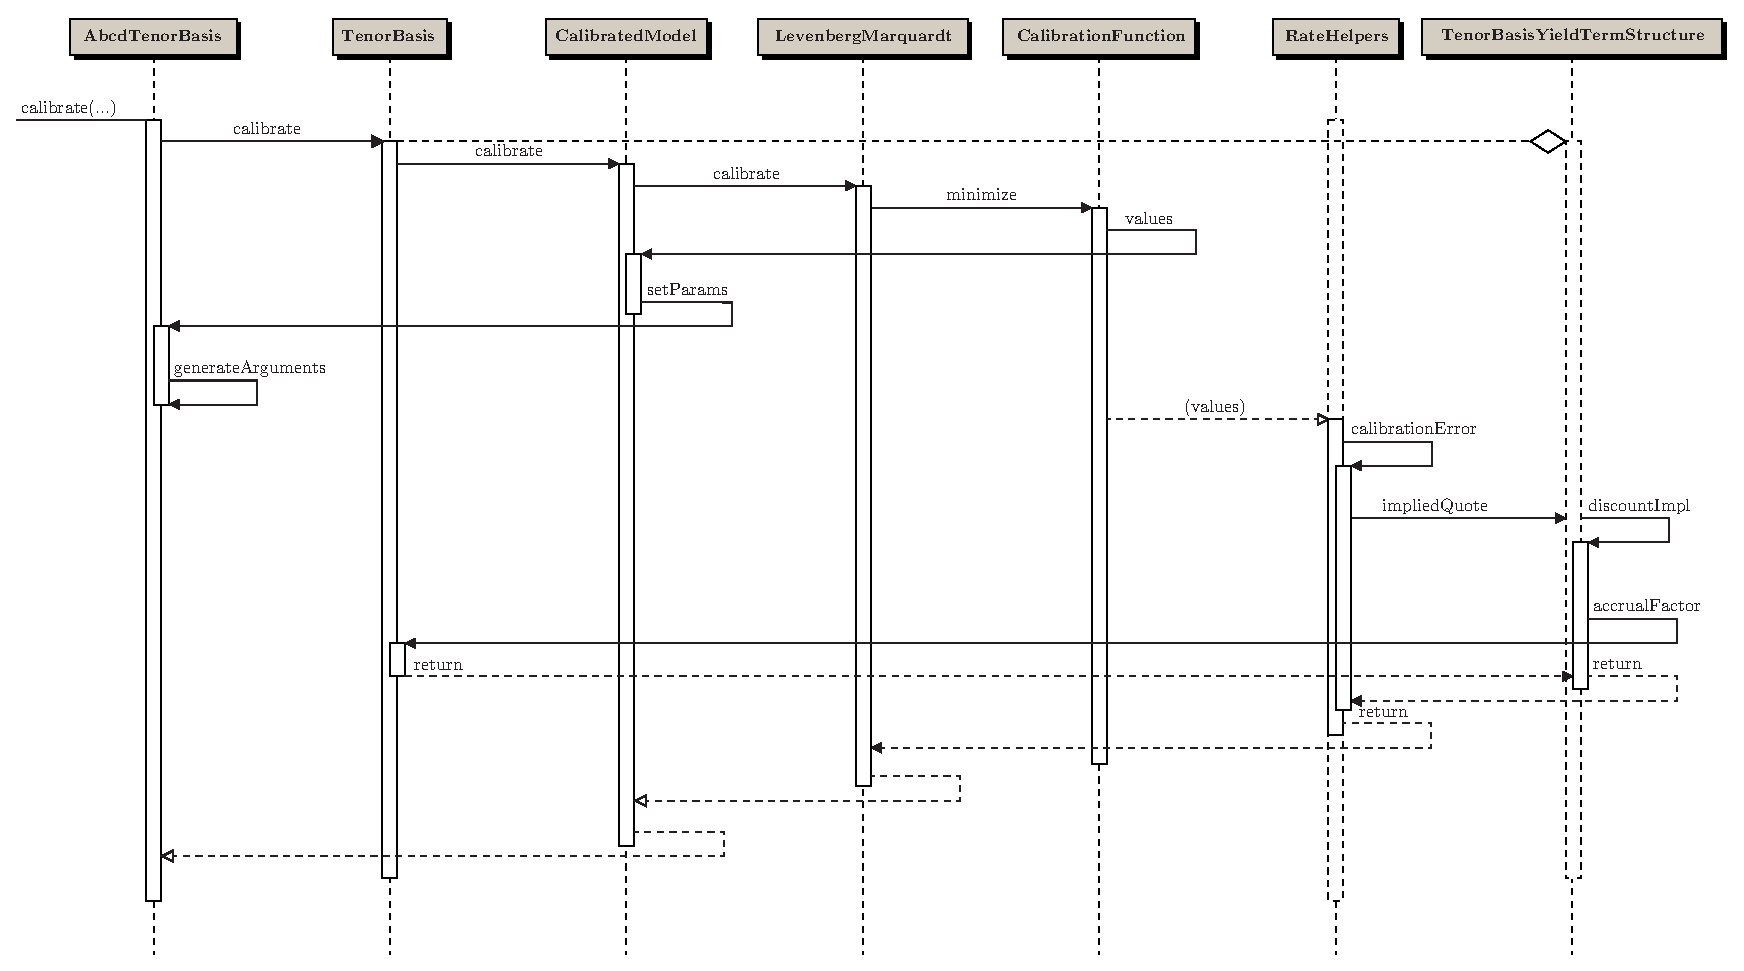
\includegraphics[angle=90,scale=0.8]{Calibrate.eps}
\caption{Calibrate}
\label{fig:calibrate}
\end{figure}

\begin{figure}[H]
\centering
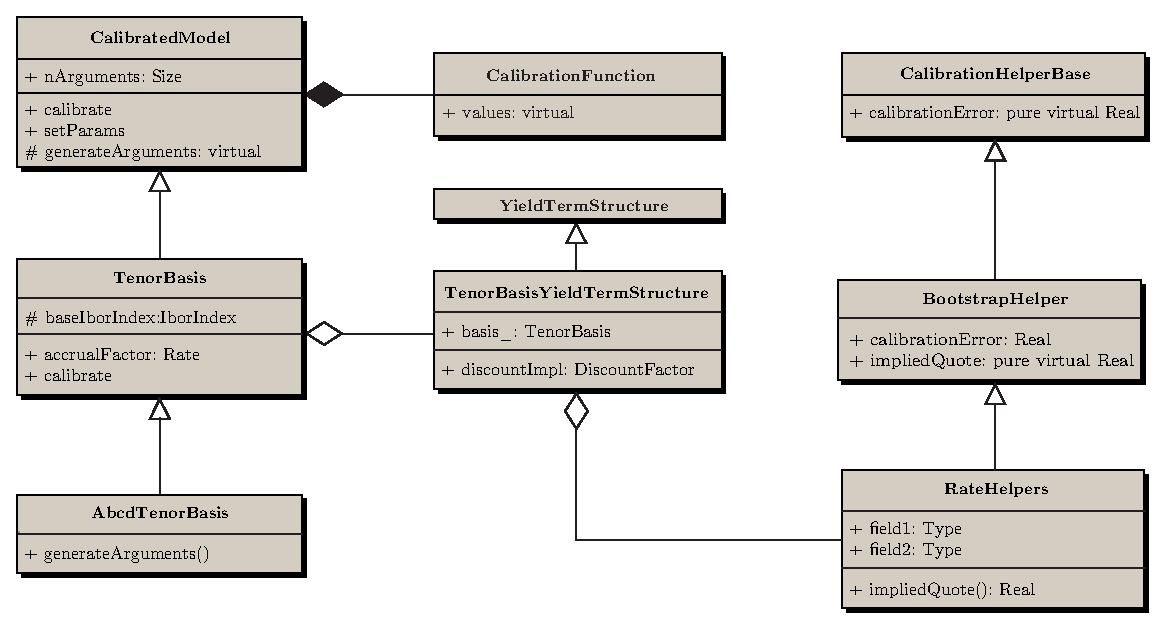
\includegraphics[scale=0.8]{Class_Tenor_Basis.eps}
\caption{Class Tenor Basis}
\label{fig:class_tenor_basis}
\end{figure}

